\chapter{ As medidas de desempenho de uma operação de produção}
\label{chap:medida_desempenho_operacao_prod}

% \section{Medidas de desempenho}
% \label{sec:sistemas_produtivos_desempenho}
Para medir corretamente o desempenho de uma operação produtiva é necessário o uso de certos indicadores. O sistema chamado \textit{Balanced Scorecard (BSC)} foi desenvolvido com este intuito e é considerado o mais equilibrado na aferição dos indicadores de desempenho da operação.
Na Figura \ref{fig:balanced_scorecard}, uma versão adaptada do BSC, baseada nos indicadores a seguir, é apresentada:

\begin{itemize}
    \item Financeiros: maior importância para proprietários e sócios da empresa;
    \item De percepção do cliente: a opinião do cliente sobre a empresa e o produto;
    \item De processos internos: a comparação com os parâmetros operacionais a serem analisados;
    \item De aprendizagem e crescimento: a competência de manter-se sustentável através de aprendizado, mudanças e melhoras ao longo do tempo.
\end{itemize}


\begin{figure}[H]
    \centering
    \caption{Balanced Scorecard (BSC)}
    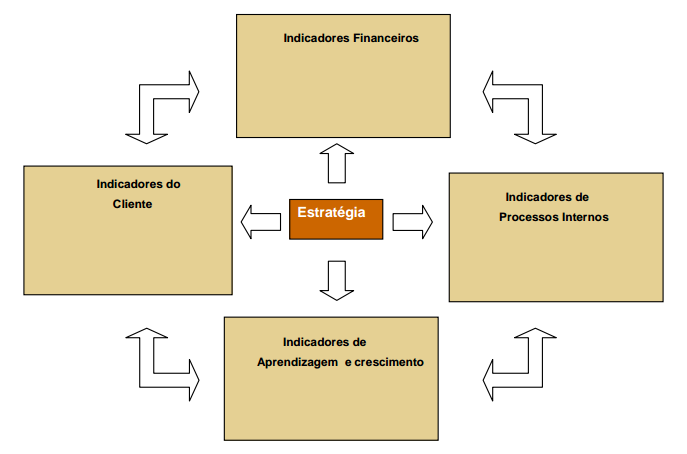
\includegraphics[width =0.8\textwidth]{images/bsc.png}
    \legend{Fonte: Adaptado de \cite{kaplan1996using}.}
    \label{fig:balanced_scorecard}
\end{figure}

O BSC é um sistema de medição de origem estratégica e seus indicadores são escolhidos de acordo com as necessidades atuais da empresa. Com o uso do sistema é esperado que se atinja o aprimoramento contínuo do negócio ao mesmo tempo que se tenha uma preocupação constante com o aprendizado e adaptação, estabelecendo novas metas para uma melhoria contínua.

Outro ponto importante a ser discutido é a diferença entre eficácia e eficiência. A primeira, representa a conquista de objetivos. Enquanto que a segunda, eficiência, é a maneira como estes objetivos são atingidos. A interpretação destes dois parâmetros de medição, é imprescindível e indissociável para a gestão de uma operação produtiva.

Reconhecendo a relevância de se medir o desempenho e entendendo a real diferença entre eficácia e eficiência, devemos listar os principais objetivos de desempenho estratégico em uma empresa industrial. %Slack (2006)
\cite{slack2006administracao} cita cinco objetivos gerais de desempenho. São eles: Qualidade, Velocidade, Flexibilidade, Confiabilidade e Custo.

\section{Aplicação prática}
\label{sec:estrategia_da_producao_aplicacao}
Dentre os possíveis indicadores de desempenho que podem ser utilizados, destacam-se aqui os de maior relevância para a SunBurn.

\textbf{Indicadores financeiros:} custo de produção por MW, custos fixos e de manutenção, bem como, tabelas tarifárias do custo da energia para o cliente final.

\textbf{Indicadores do cliente:} o cliente, que é uma empresa de distribuição de energia elétrica, pode utilizar os indicadores de qualidade definidos pela \ac{ANEEL} como base para formar sua opinião sobre o produto entregue pela SunBurn.

\textbf{Indicadores de aprendizagem e crescimento:} desenvolvimento de melhorias de processo produtivo e de manutenção.

\textbf{Indicadores de processos internos:} baseados nos indicadores especificados pelas instruções normativas da \ac{ANEEL}, tais como indicadores de qualidade do produto (conformidade de tensão em regime permanente e perturbações na forma de onda de tensão) \cite{ANEEL_Produto}, indicadores de conformidade da entrega da energia contratada \cite{ANEEL_Continuidade} e indicadores de segurança do trabalho e das instalações \cite{ANEEL_Seguranca}. Ressalta-se que estes indicadores estão definidos no \textit{site} da \ac{ANEEL} para as empresas distribuidoras de energia elétrica, as quais são clientes da SunBurn, logo tais indicadores podem e devem ser adaptados para esta empresa.
